%-----------------------------------------------------------------------------------------------%
%
% Maret 2019
% Template Latex untuk Tugas Akhir Program Studi Sistem informasi ini
% dikembangkan oleh Inggih Permana (inggihjava@gmail.com)
%
% Template ini dikembangkan dari template yang dibuat oleh Andreas Febrian (Fasilkom UI 2003).
%
% Orang yang cerdas adalah orang yang paling banyak mengingat kematian.
%
%-----------------------------------------------------------------------------------------------%

%-----------------------------------------------------------------------------%
%\prefikLampiran{A}
\renewcommand{\thepage}{A - \arabic{page}}
\chapter{HASIL WAWANCARA}

\begin{figure}[h]
	\centering
	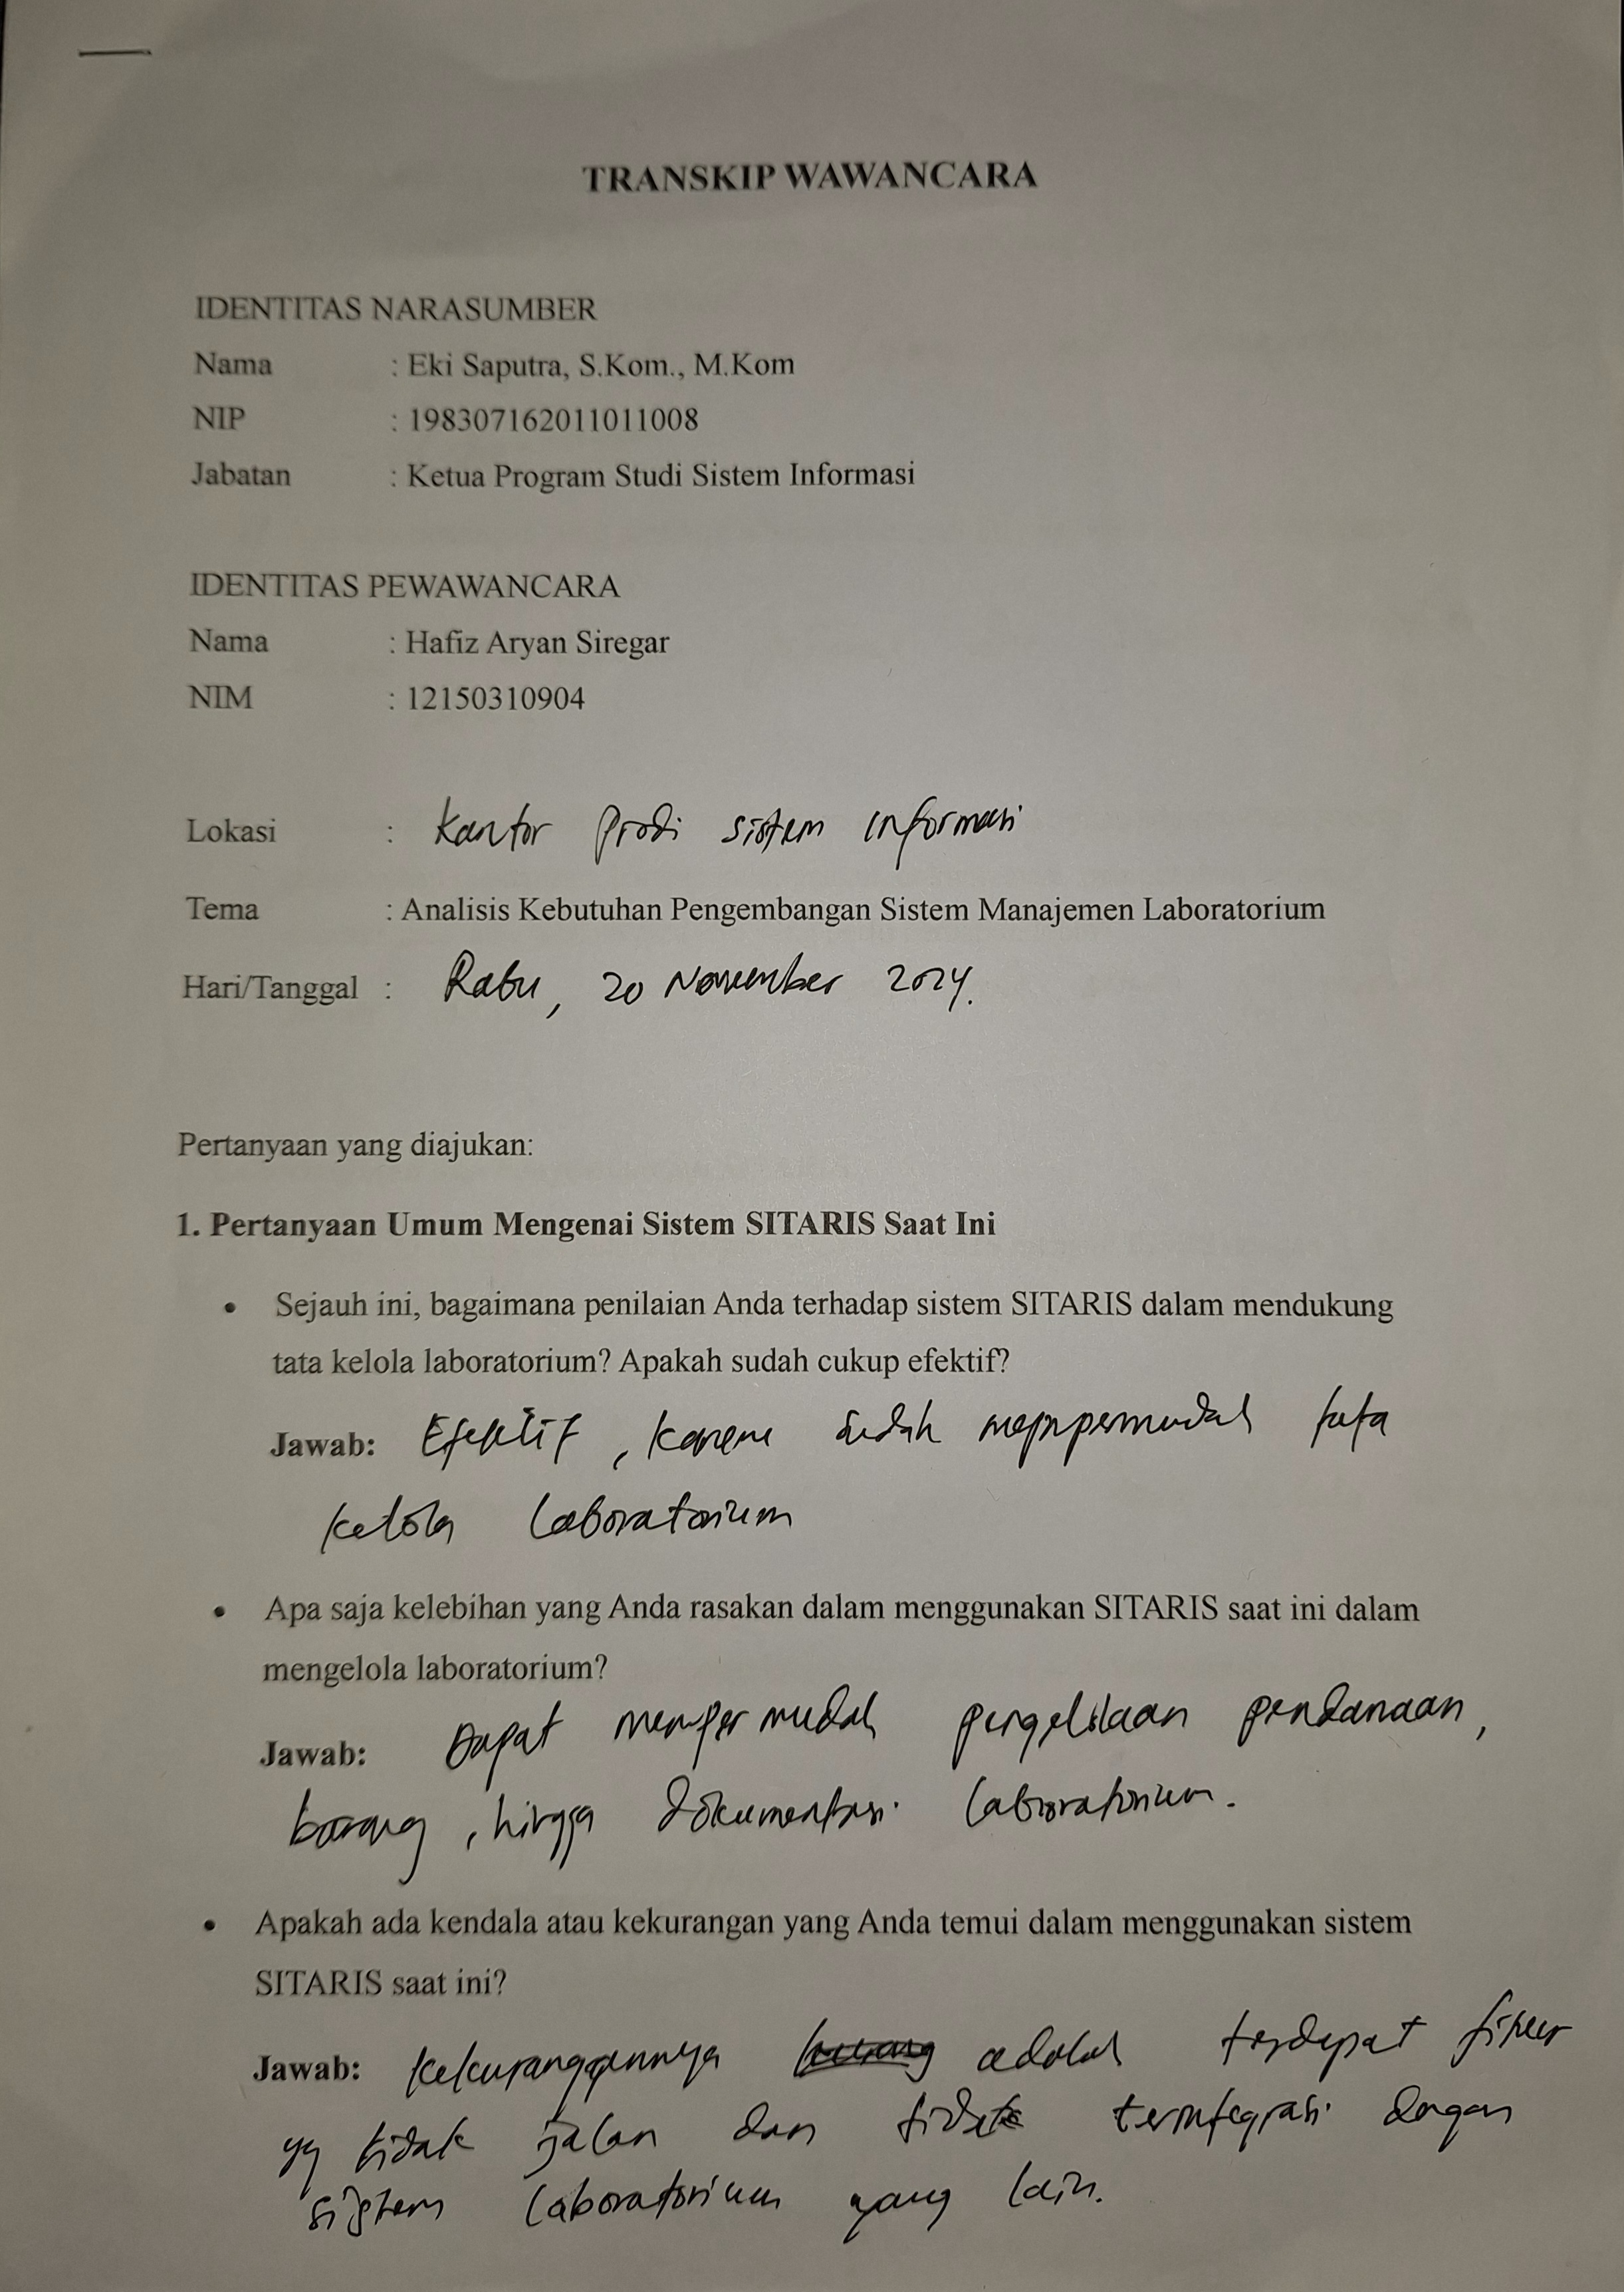
\includegraphics[width=0.82\linewidth]{konten/gambar/wawancara/1.jpg}
	\caption{Transkip Wawancara Kaprodi}
	\label{fig:hasil-wawancara}
\end{figure}
\begin{figure}[h]
	\centering
	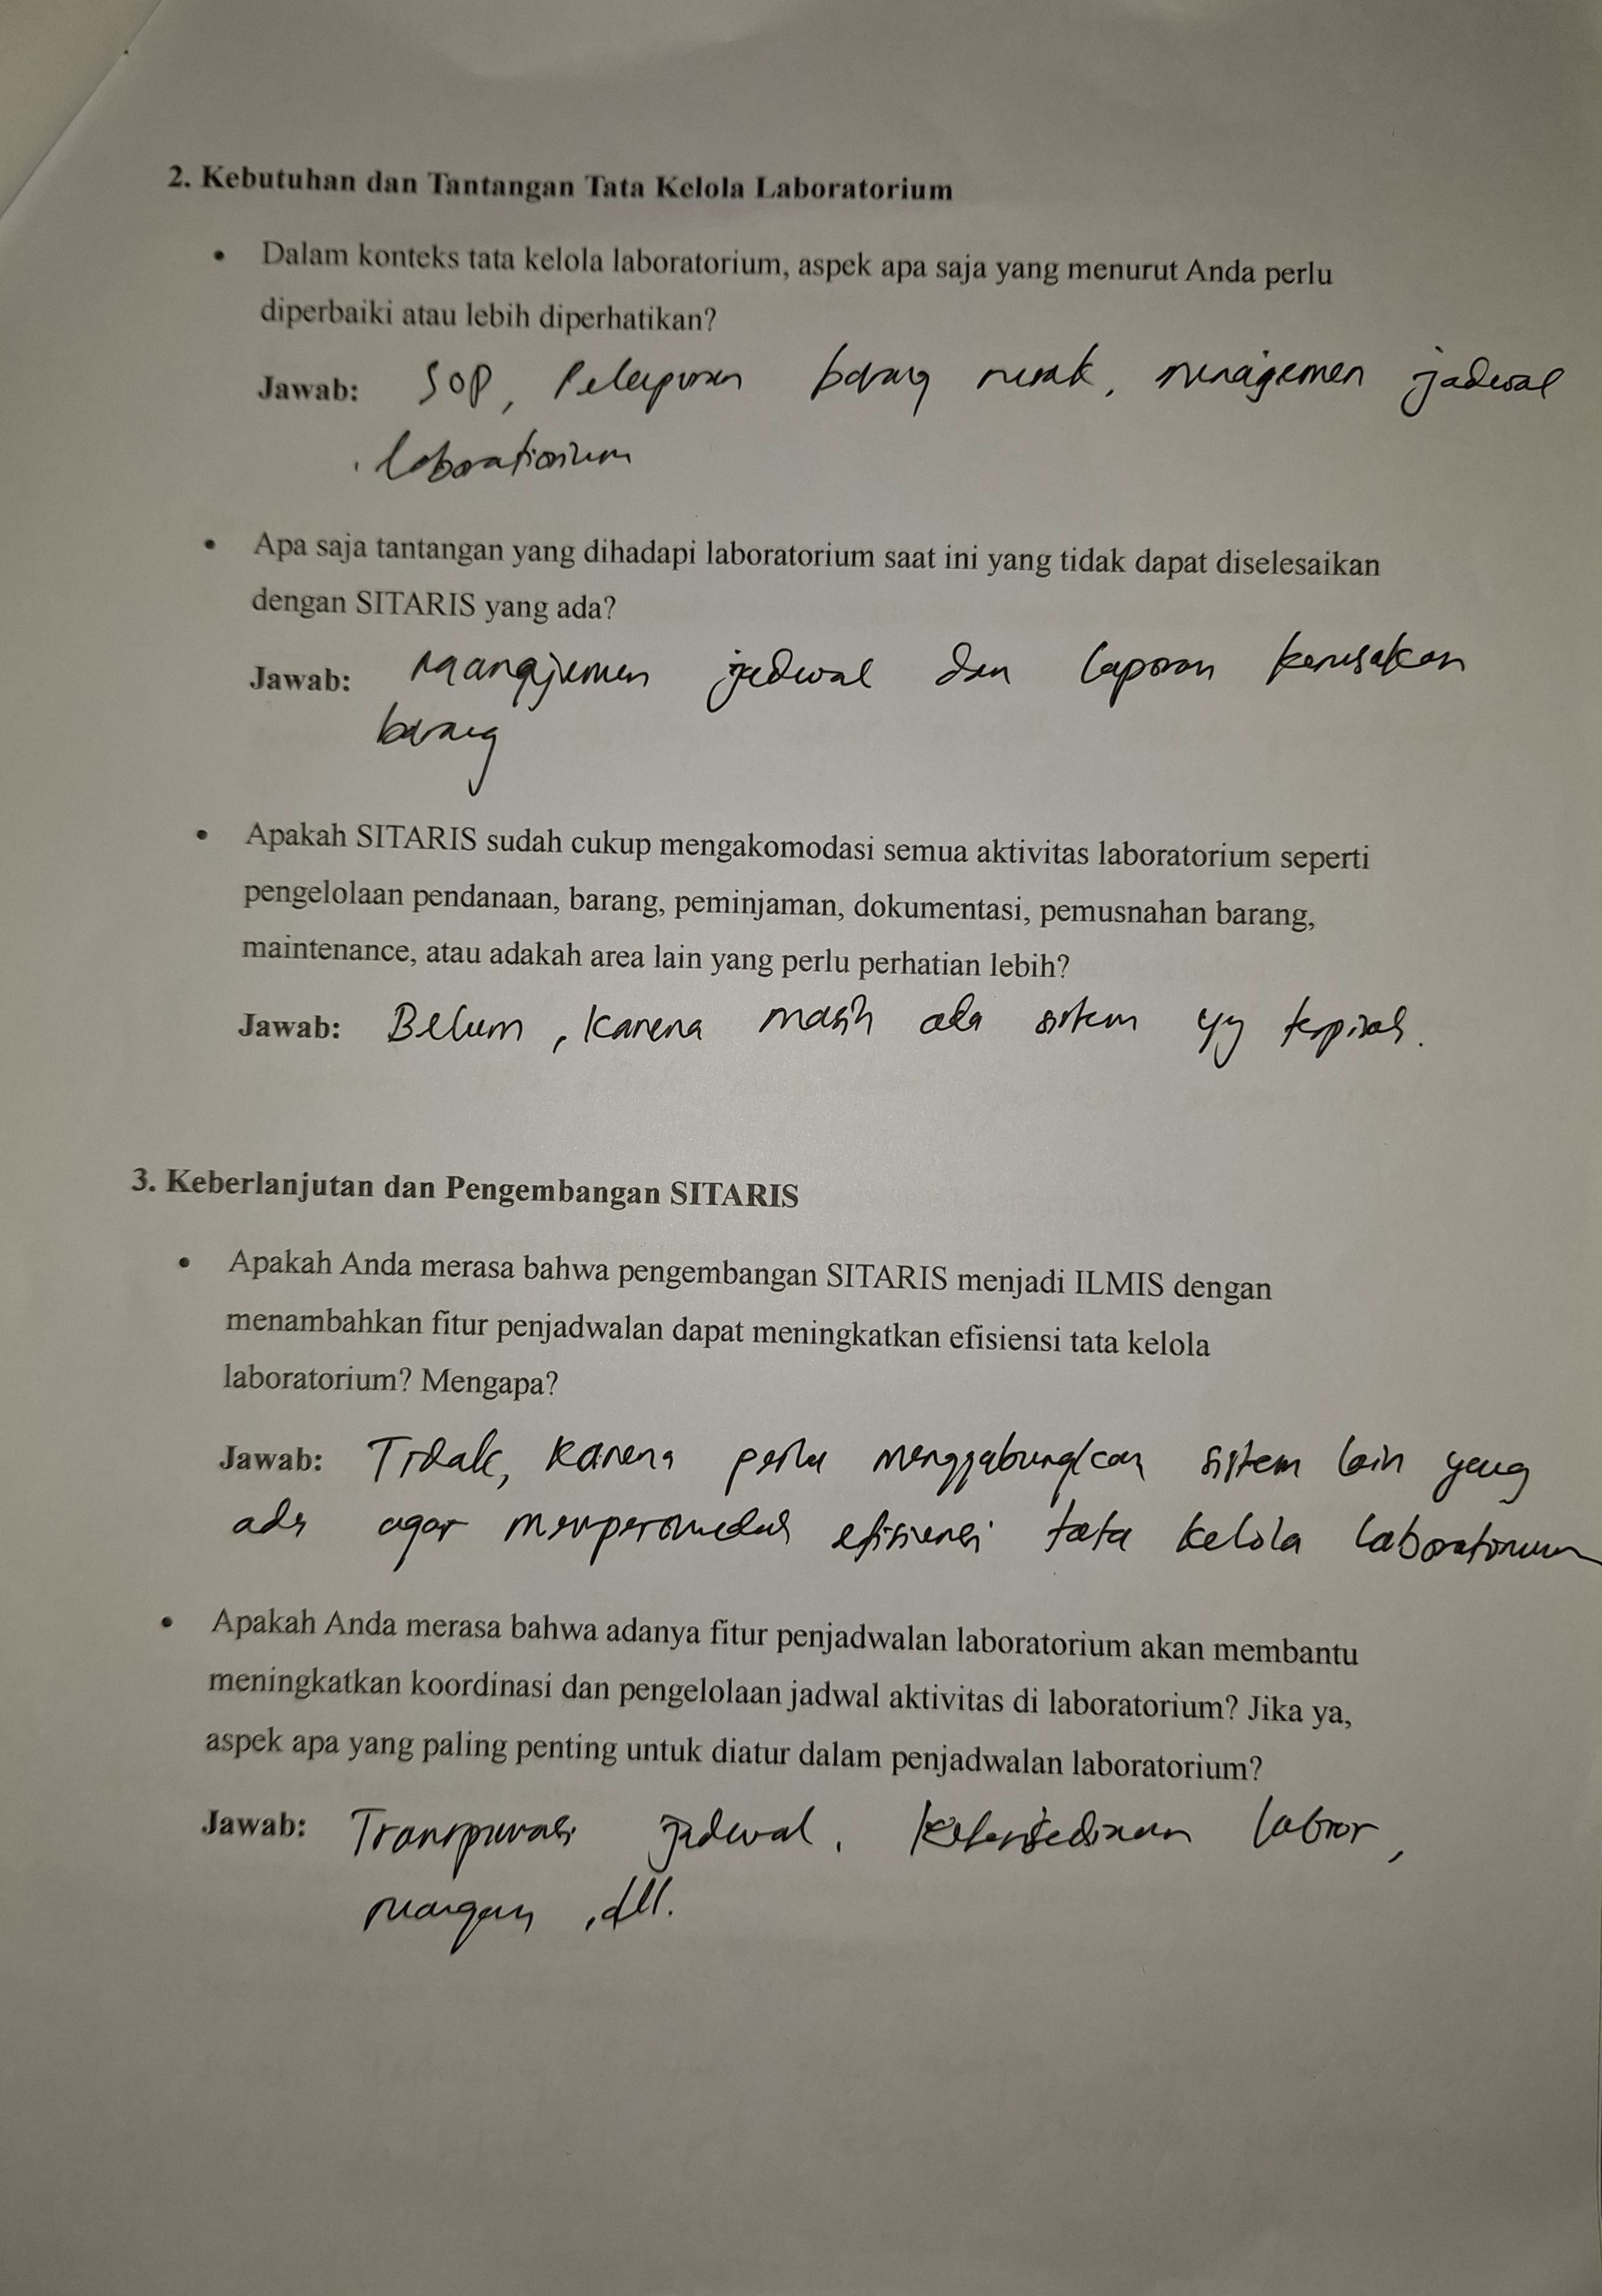
\includegraphics[width=0.82\linewidth]{konten/gambar/wawancara/2.jpg}

	\label{fig:hasil-wawancara}
\end{figure}
\begin{figure}[h]
	\centering
	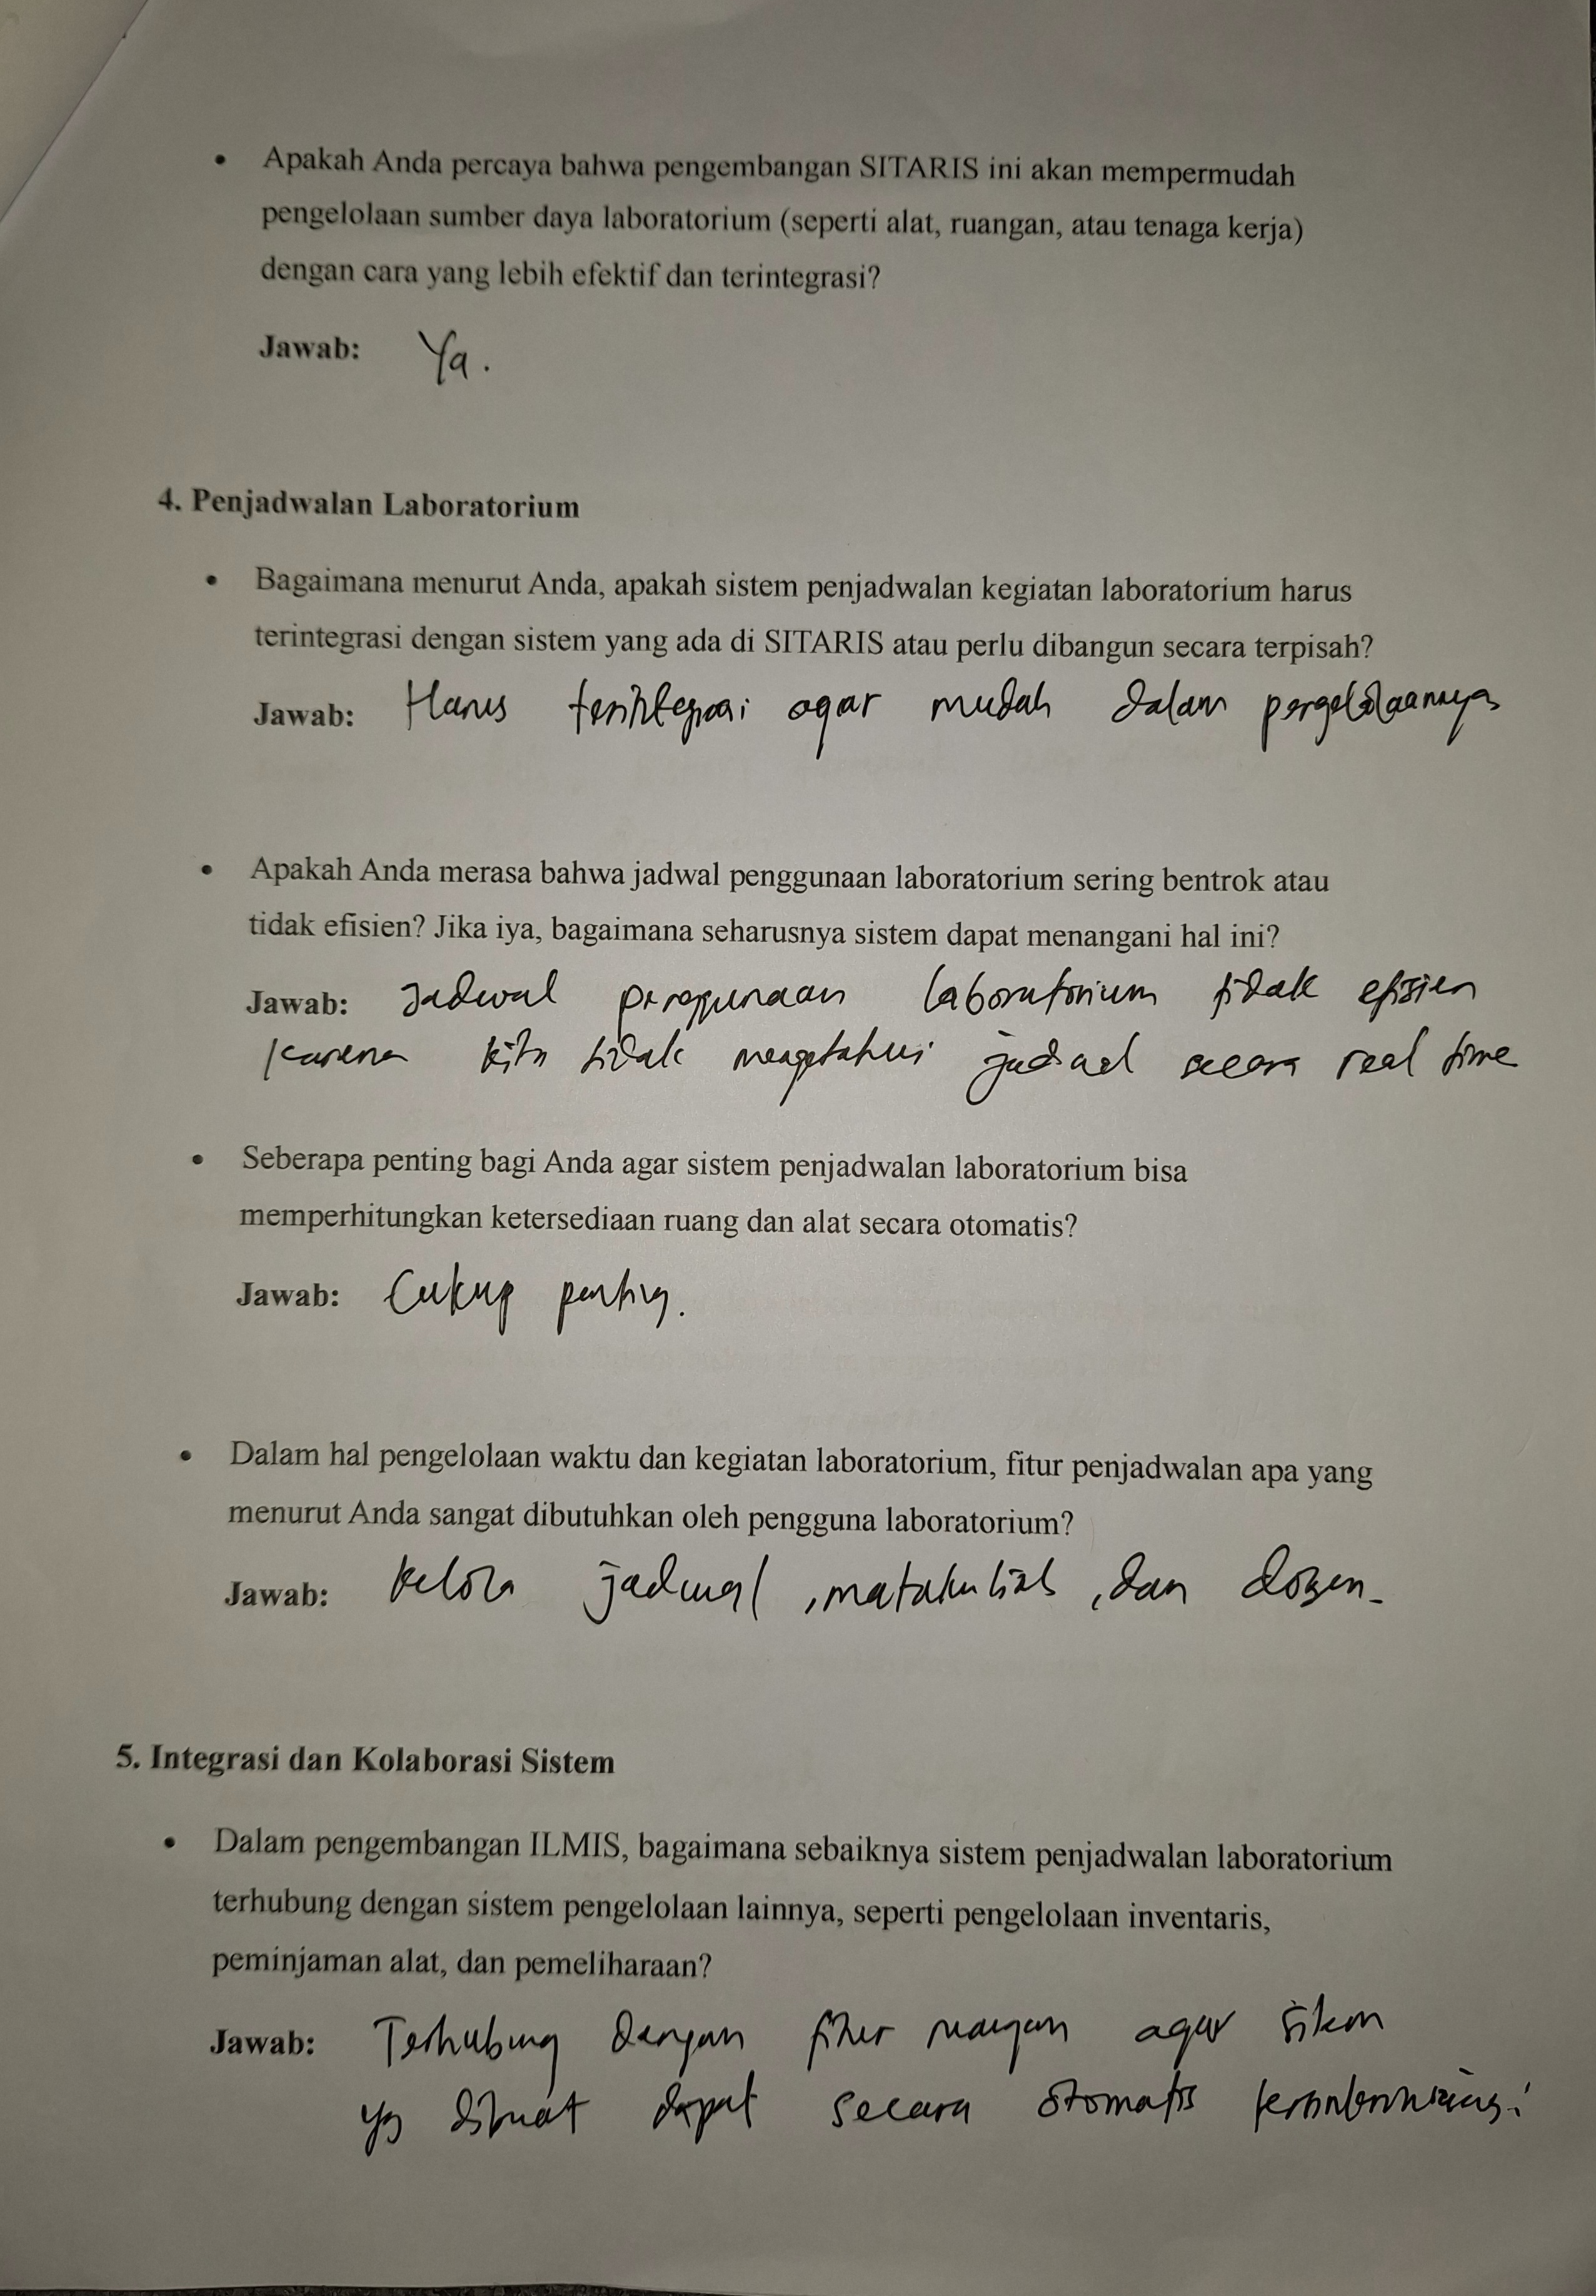
\includegraphics[width=0.82\linewidth]{konten/gambar/wawancara/3.jpg}

	\label{fig:hasil-wawancara}
\end{figure}
\begin{figure}[h]
	\centering
	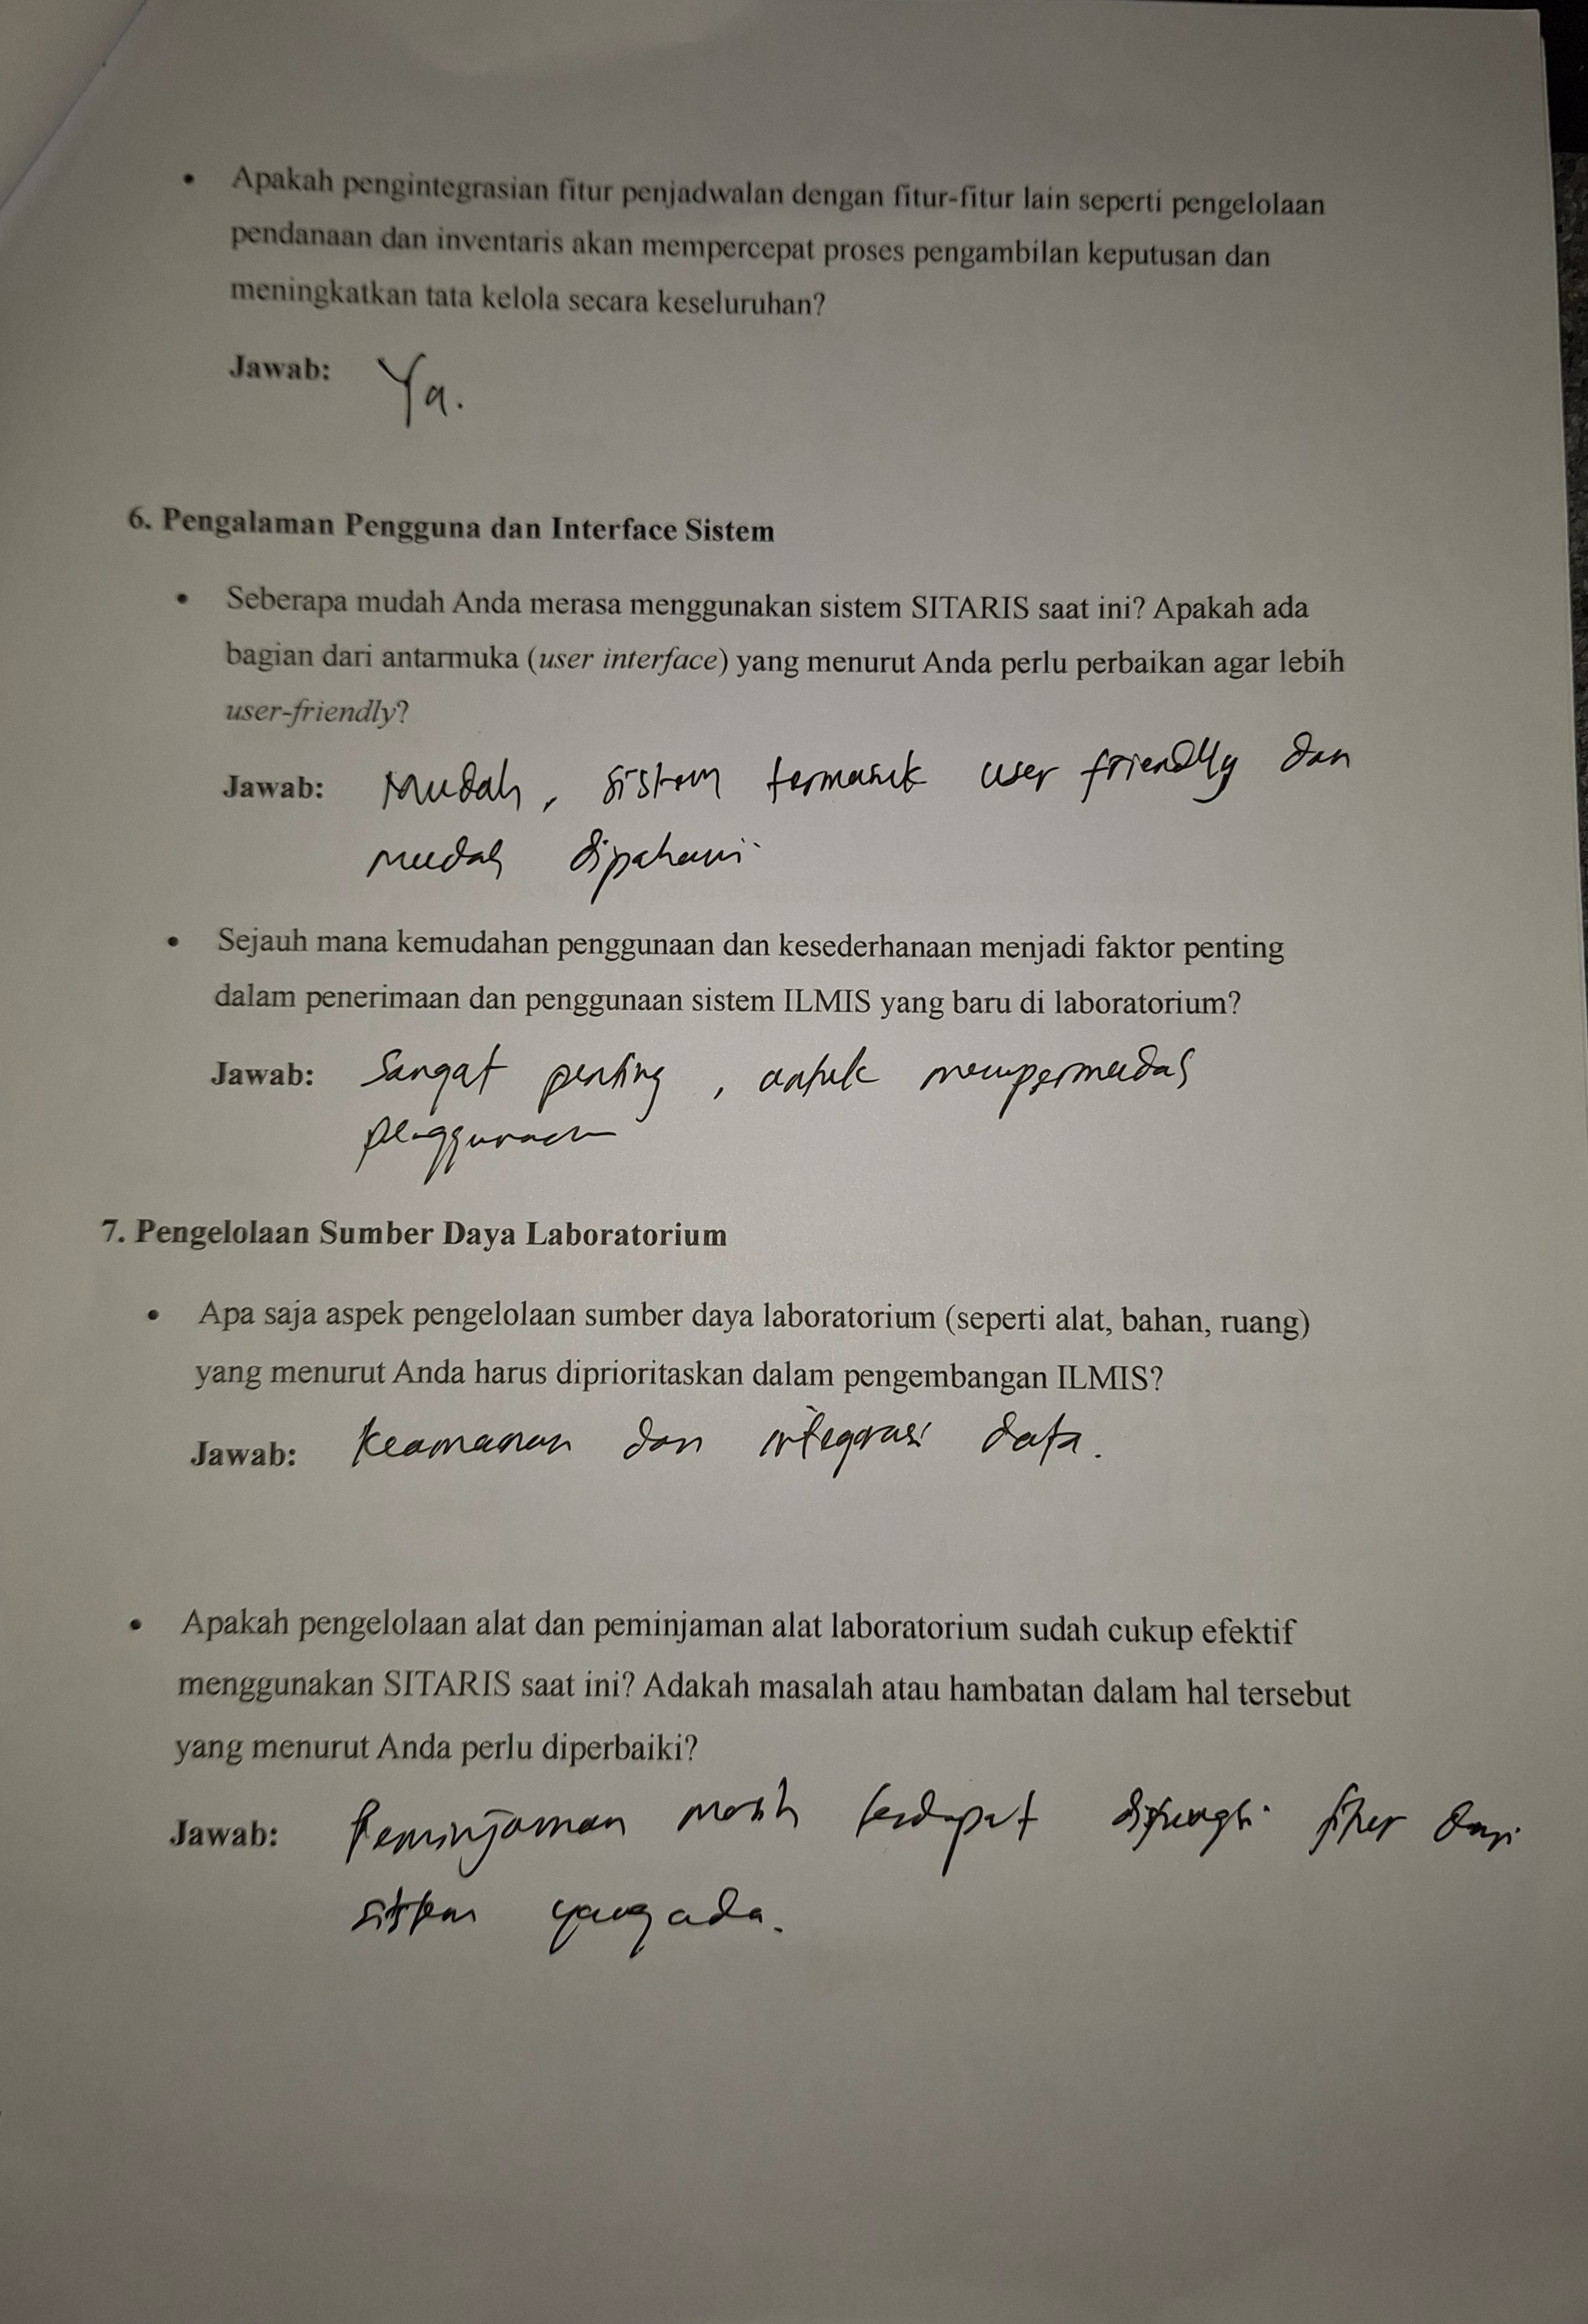
\includegraphics[width=0.82\linewidth]{konten/gambar/wawancara/4.jpg}

	\label{fig:hasil-wawancara}
\end{figure}
\begin{figure}[h]
	\centering
	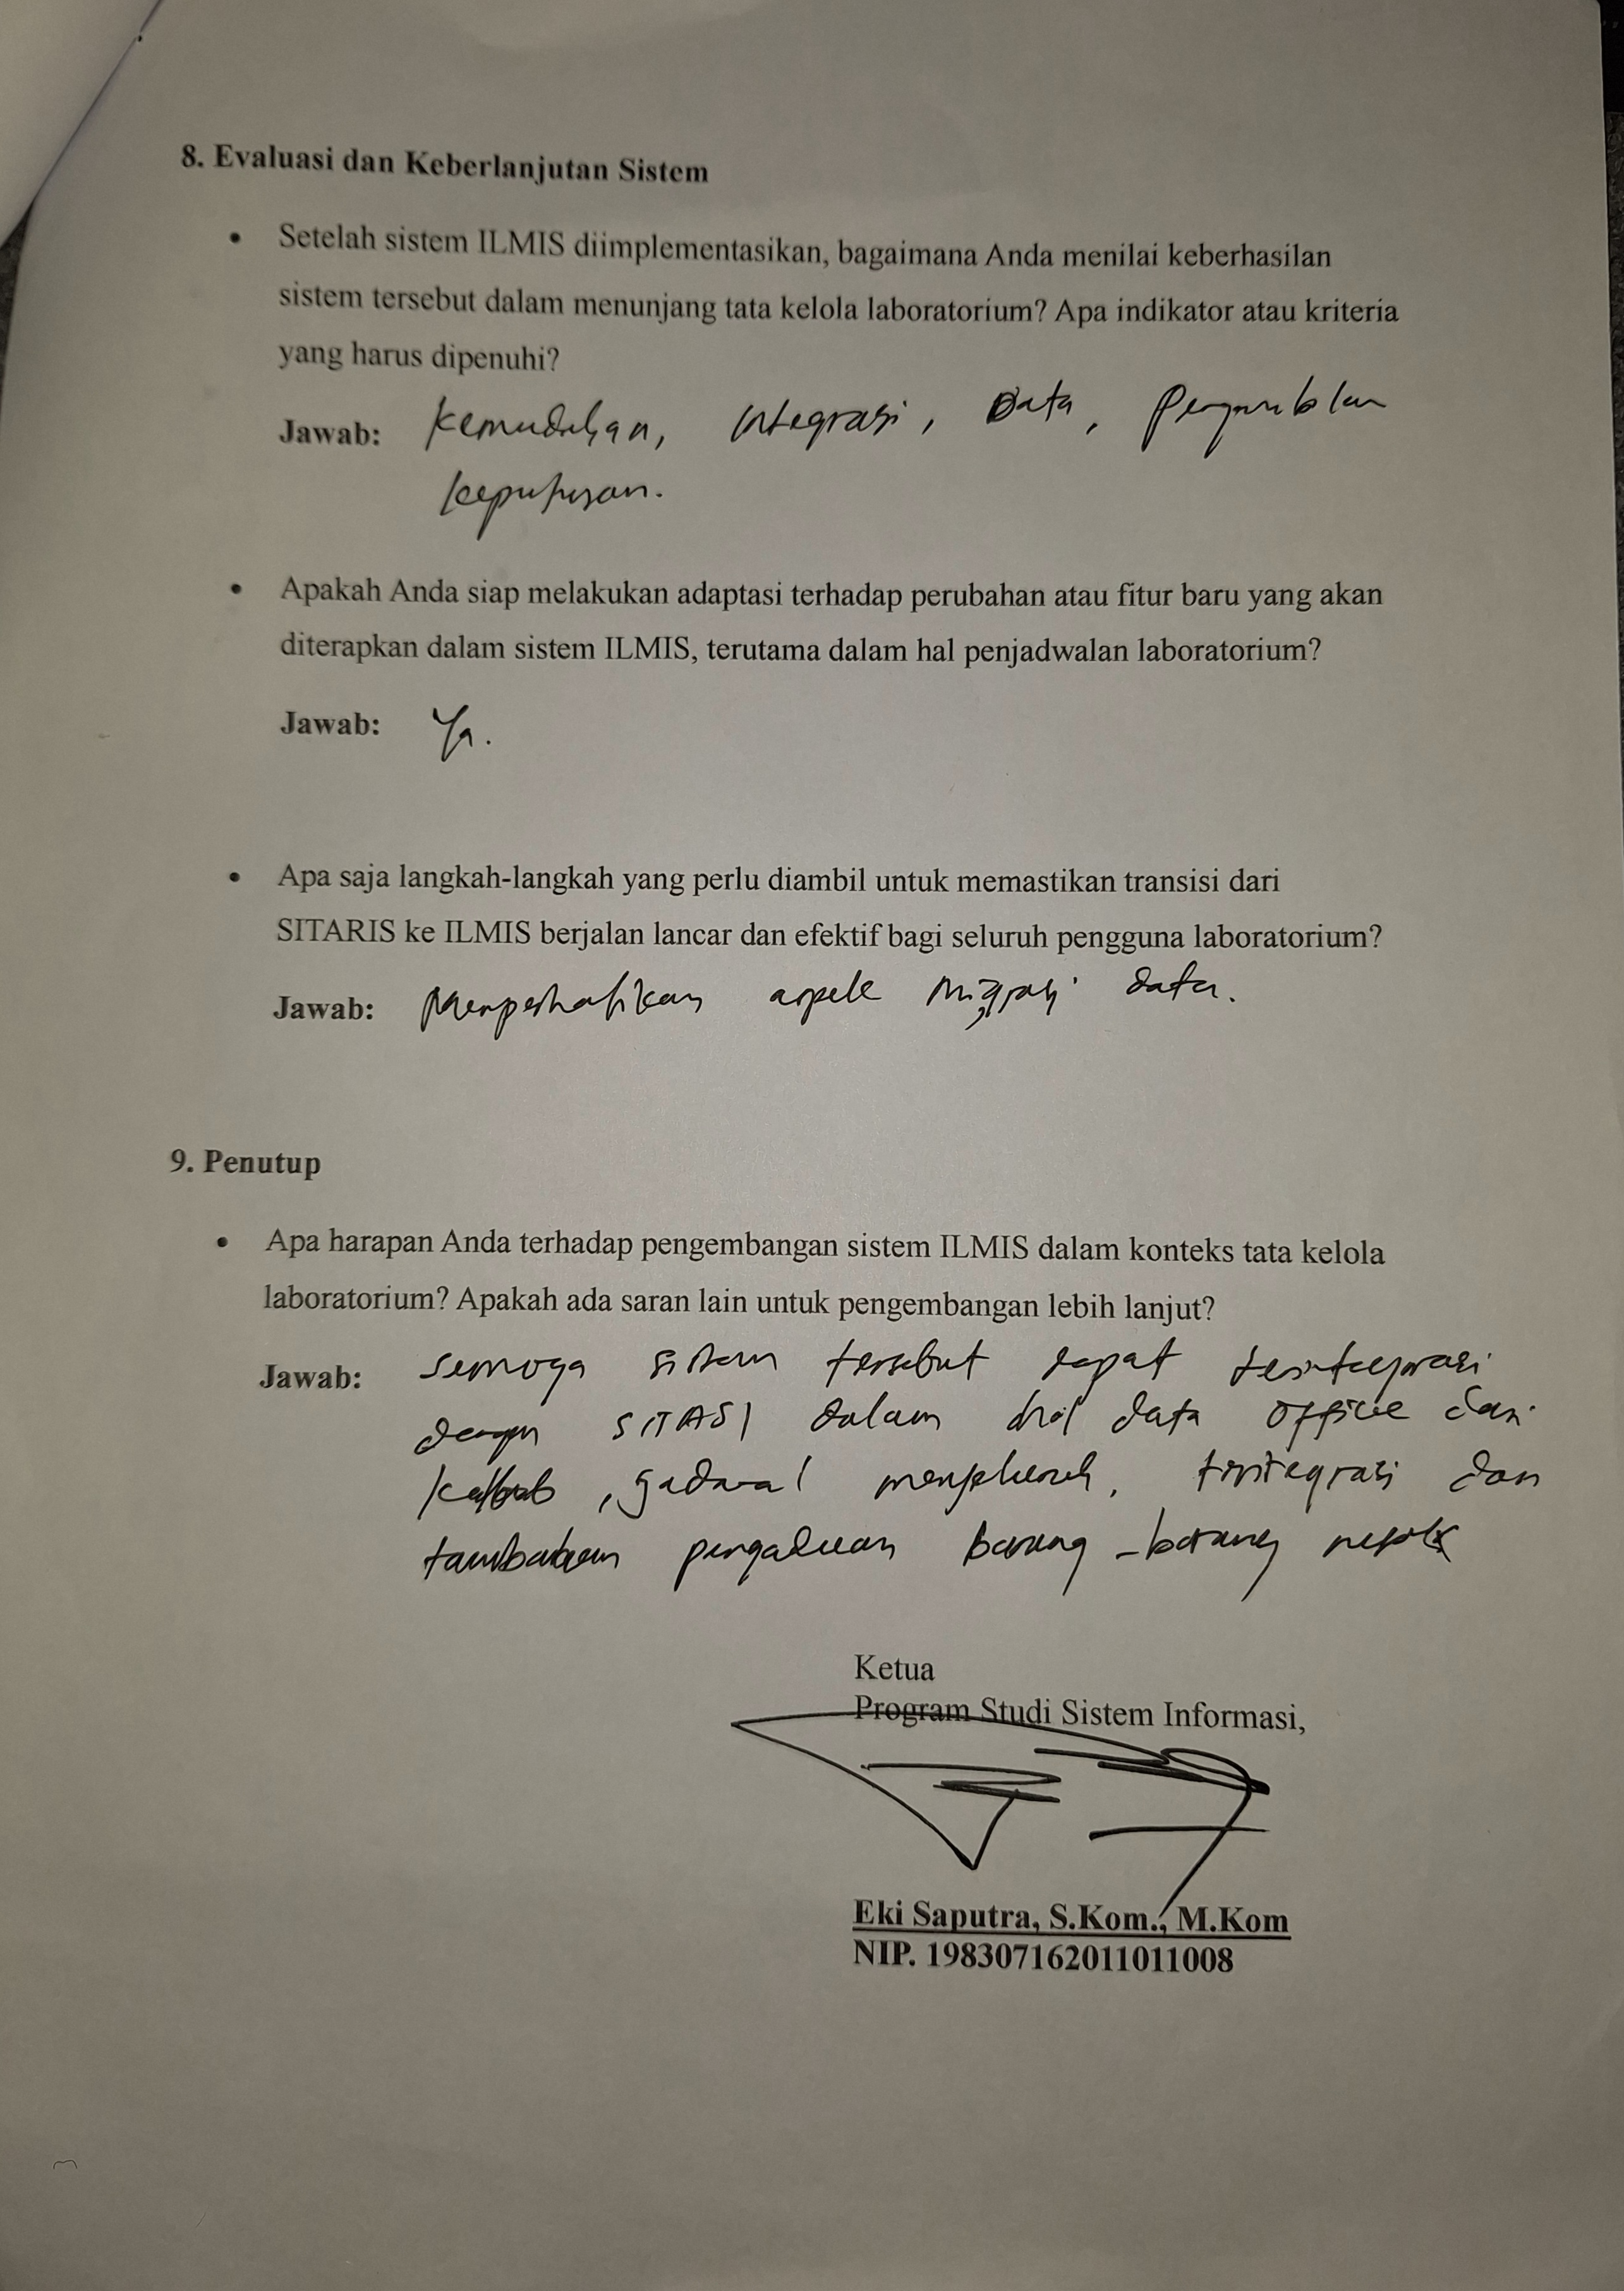
\includegraphics[width=0.82\linewidth]{konten/gambar/wawancara/5.jpg}

	\label{fig:hasil-wawancara}
\end{figure}
\begin{figure}[h]
	\centering
	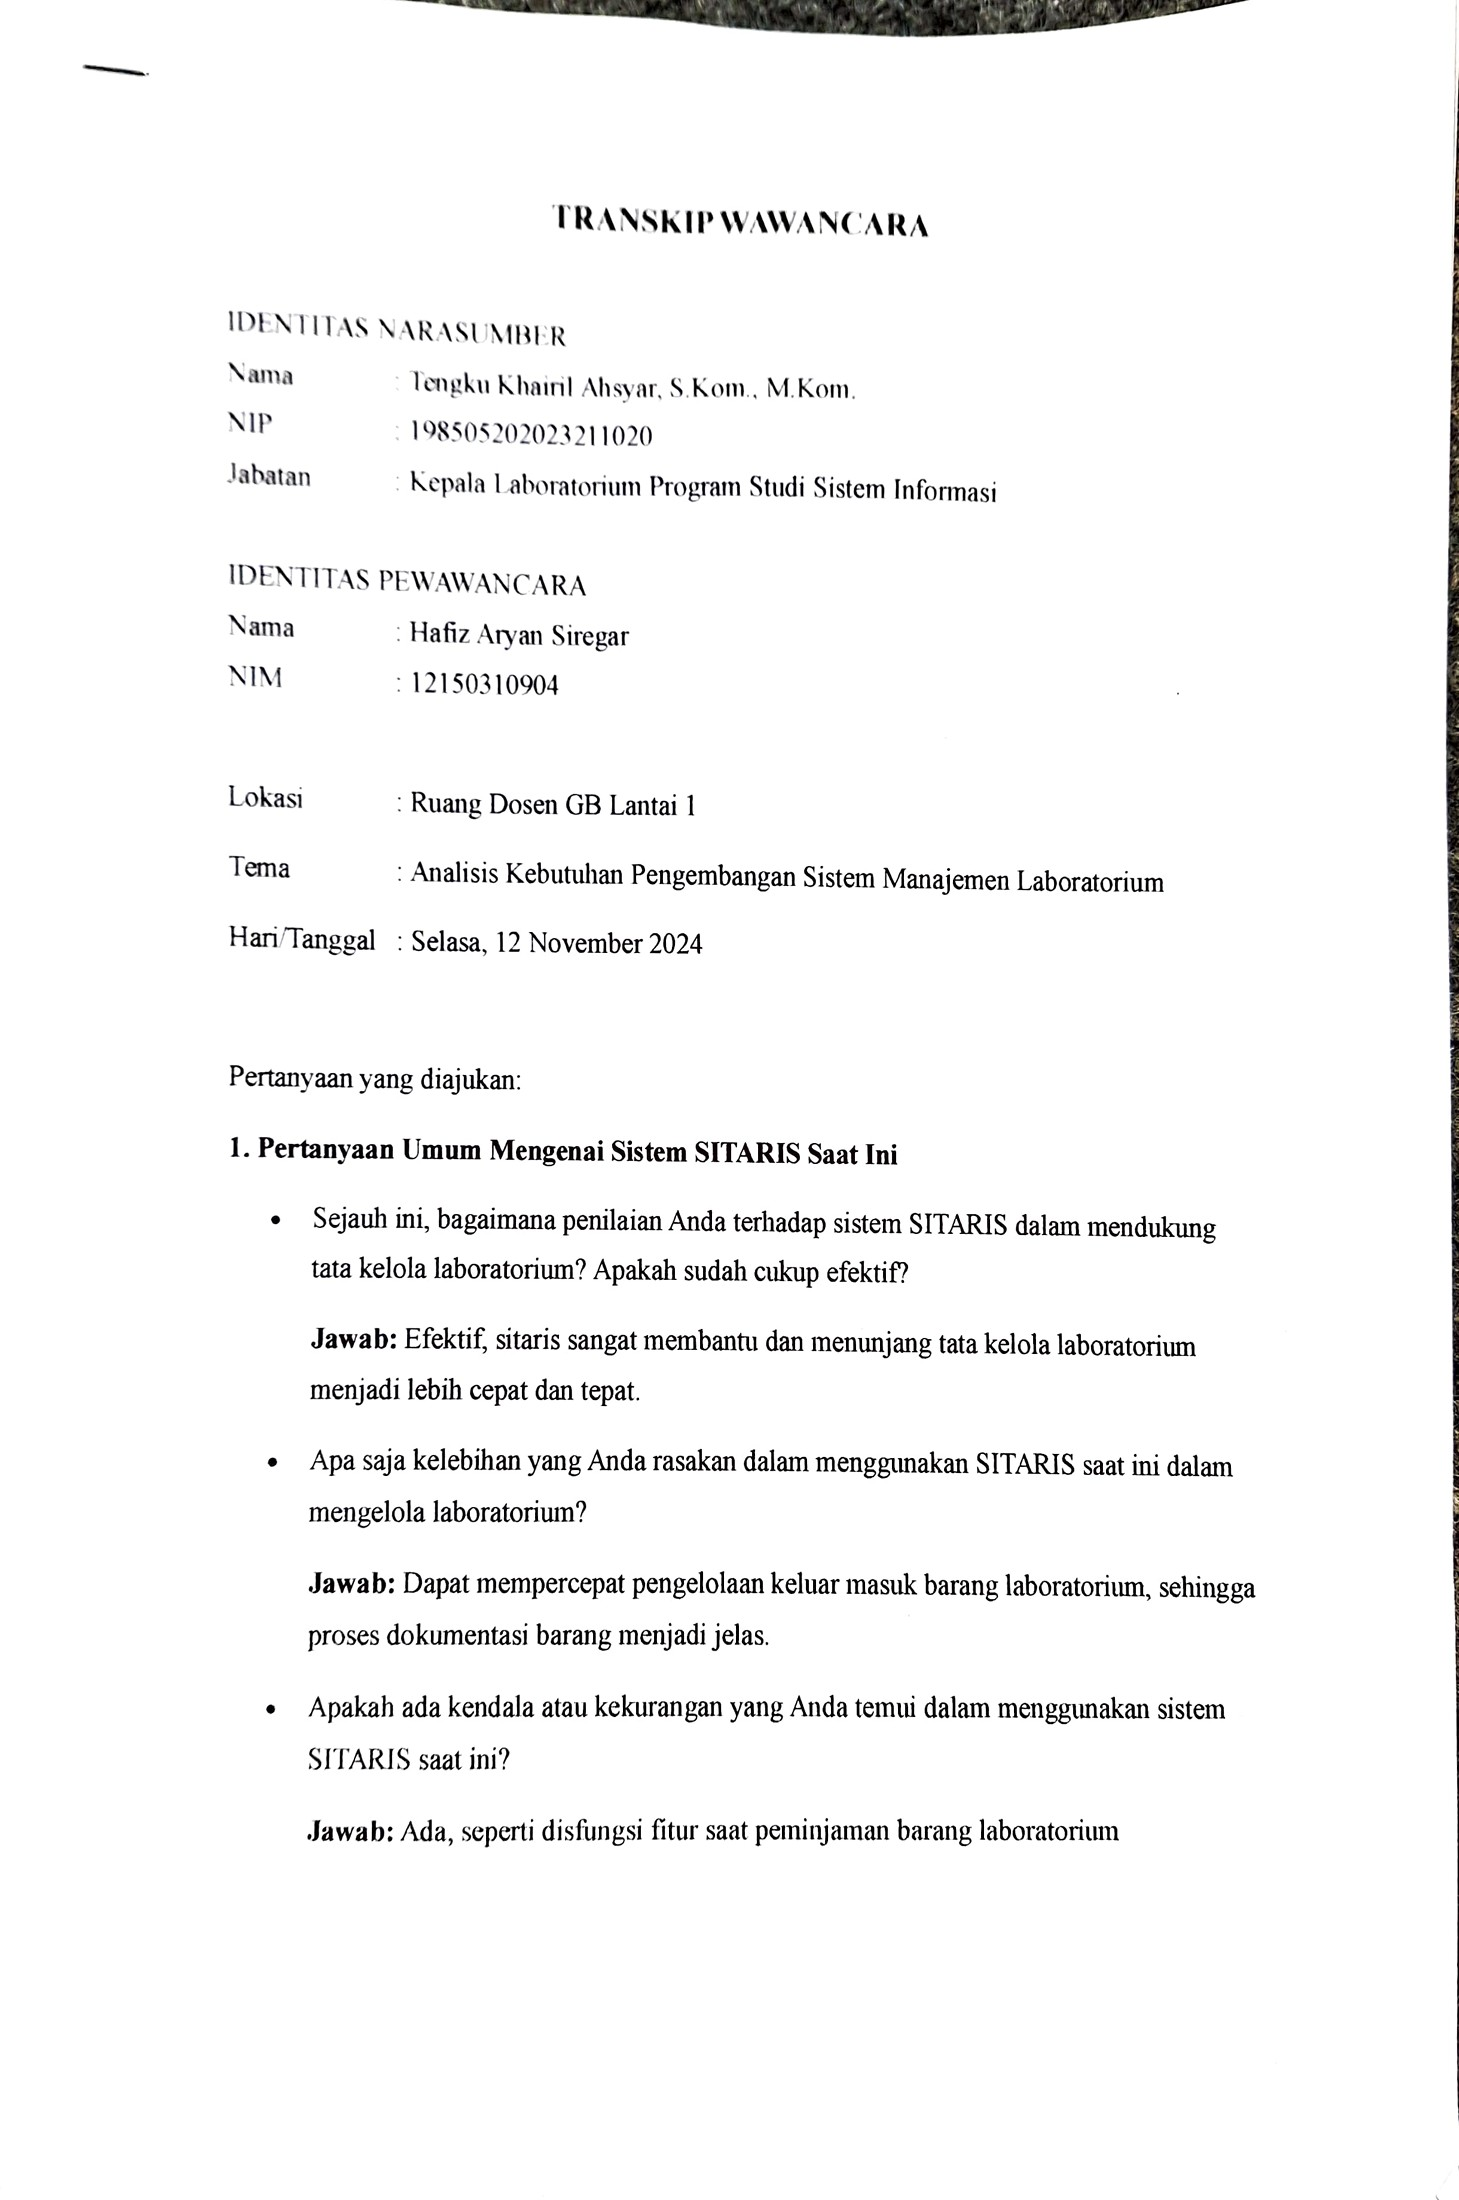
\includegraphics[width=0.82\linewidth]{konten/gambar/wawancara/wawancara_1.jpg}
	\caption{Transkip Wawancara Kalab}
	\label{fig:hasil-wawancara}
\end{figure}
\begin{figure}[h]
	\centering
	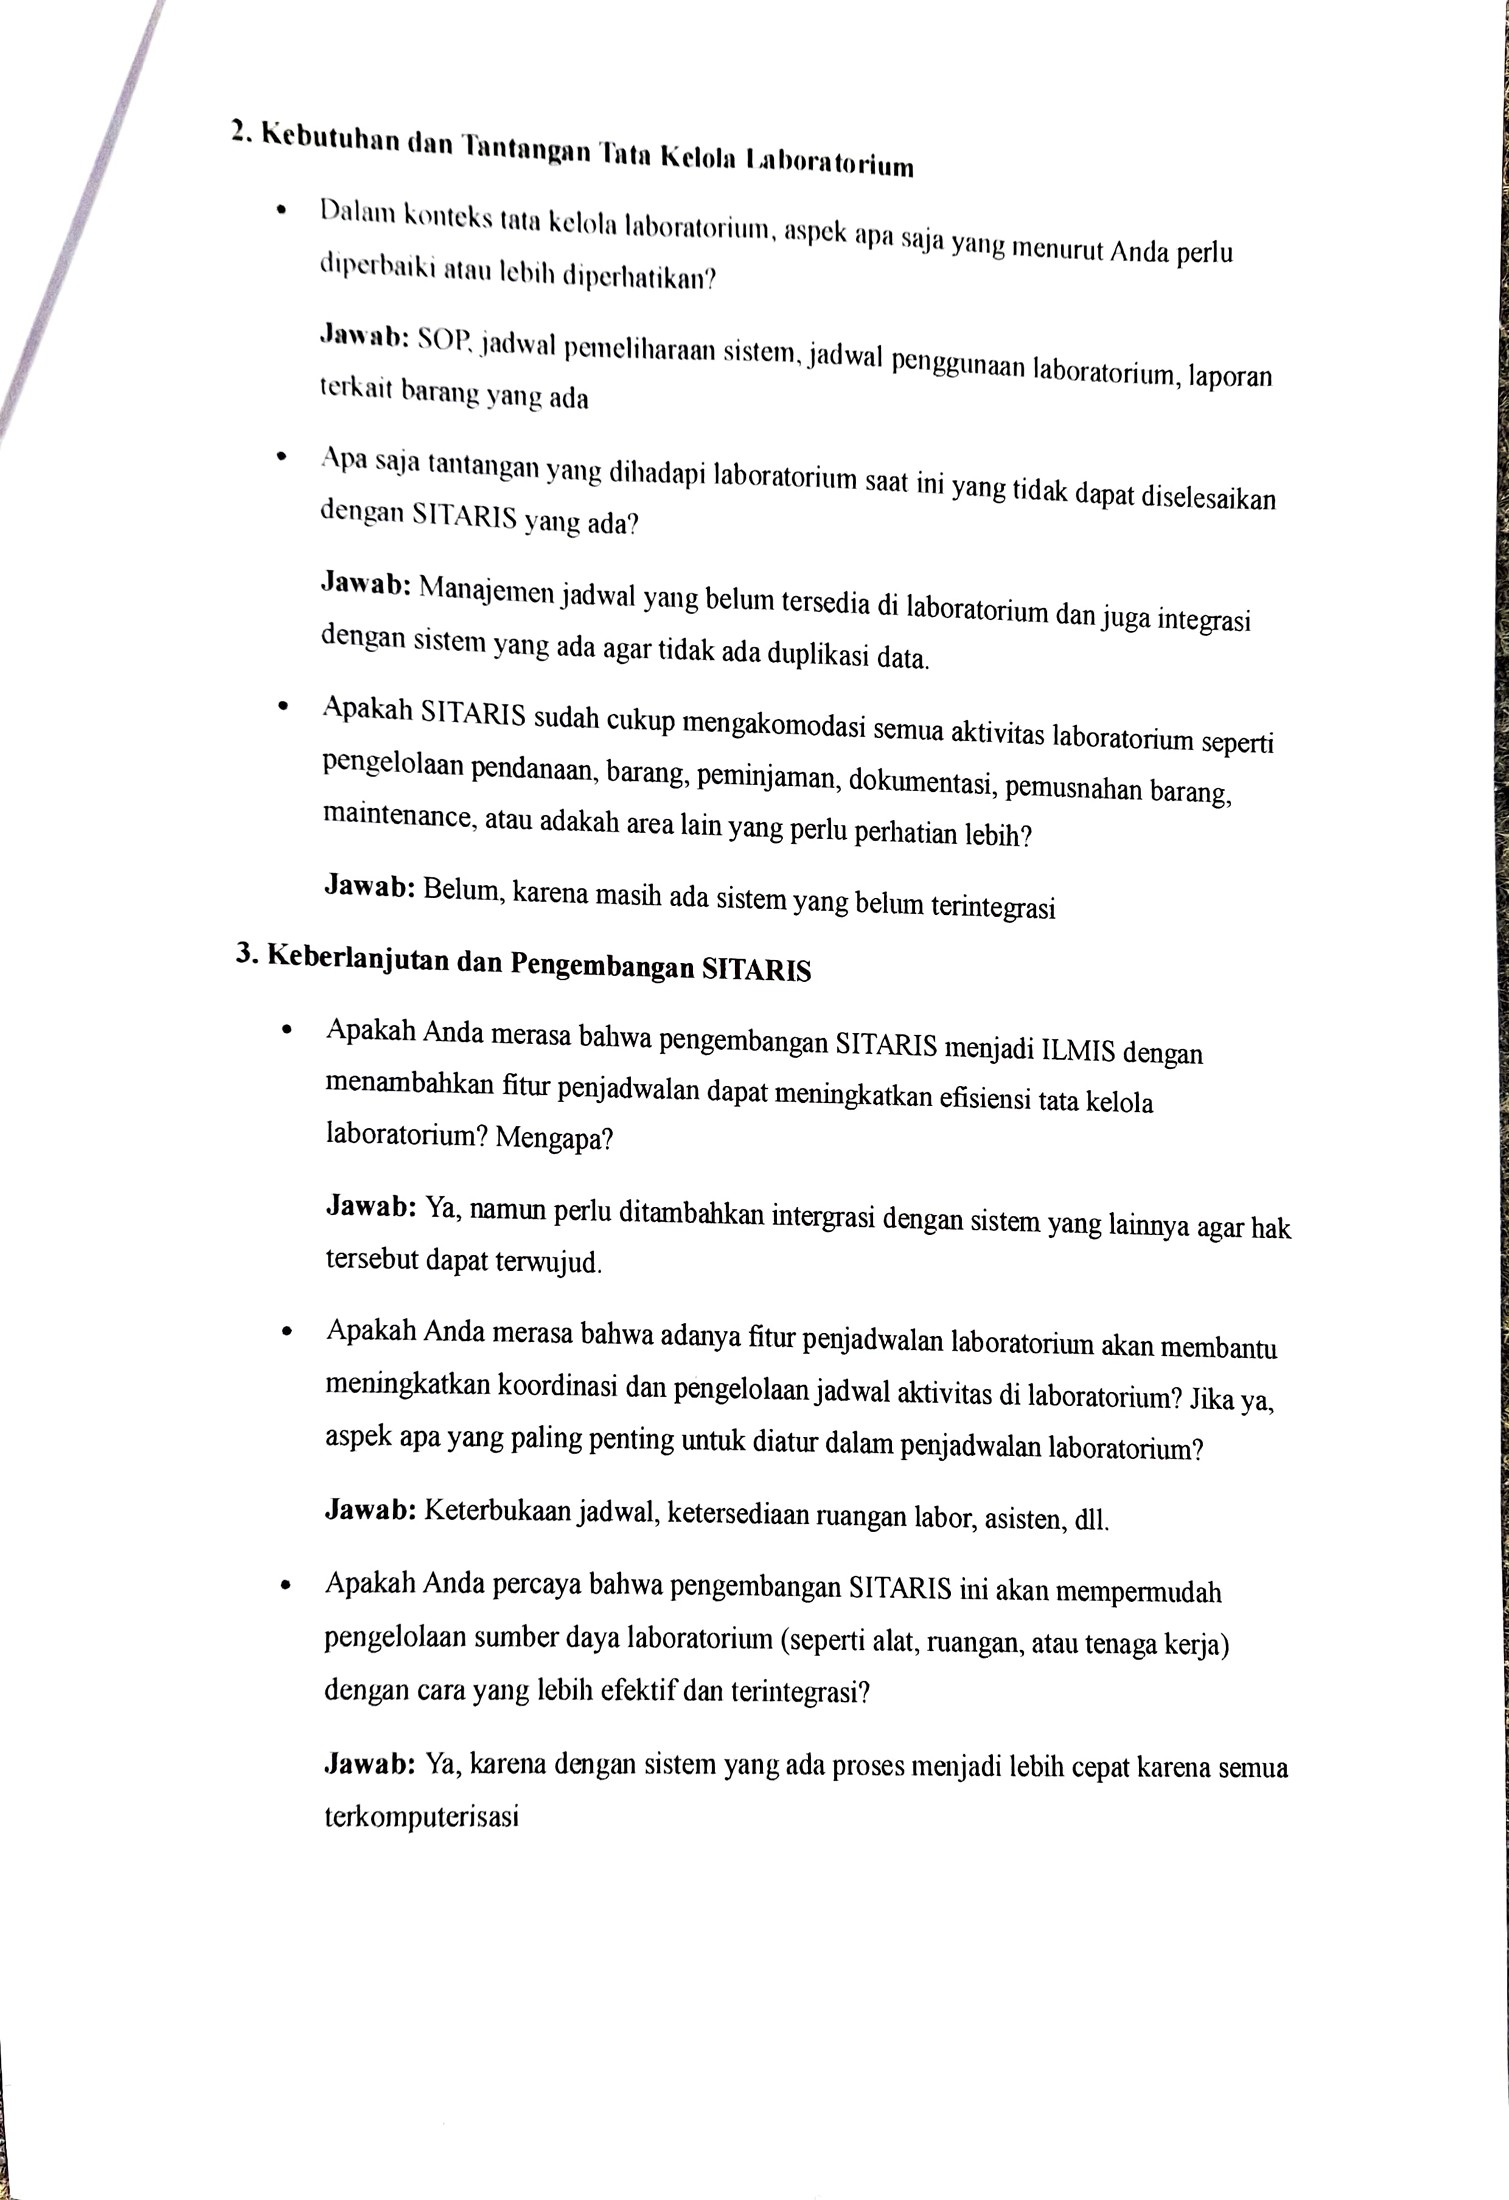
\includegraphics[width=0.82\linewidth]{konten/gambar/wawancara/wawancara_2.jpg}

	\label{fig:hasil-wawancara}
\end{figure}
\begin{figure}[h]
	\centering
	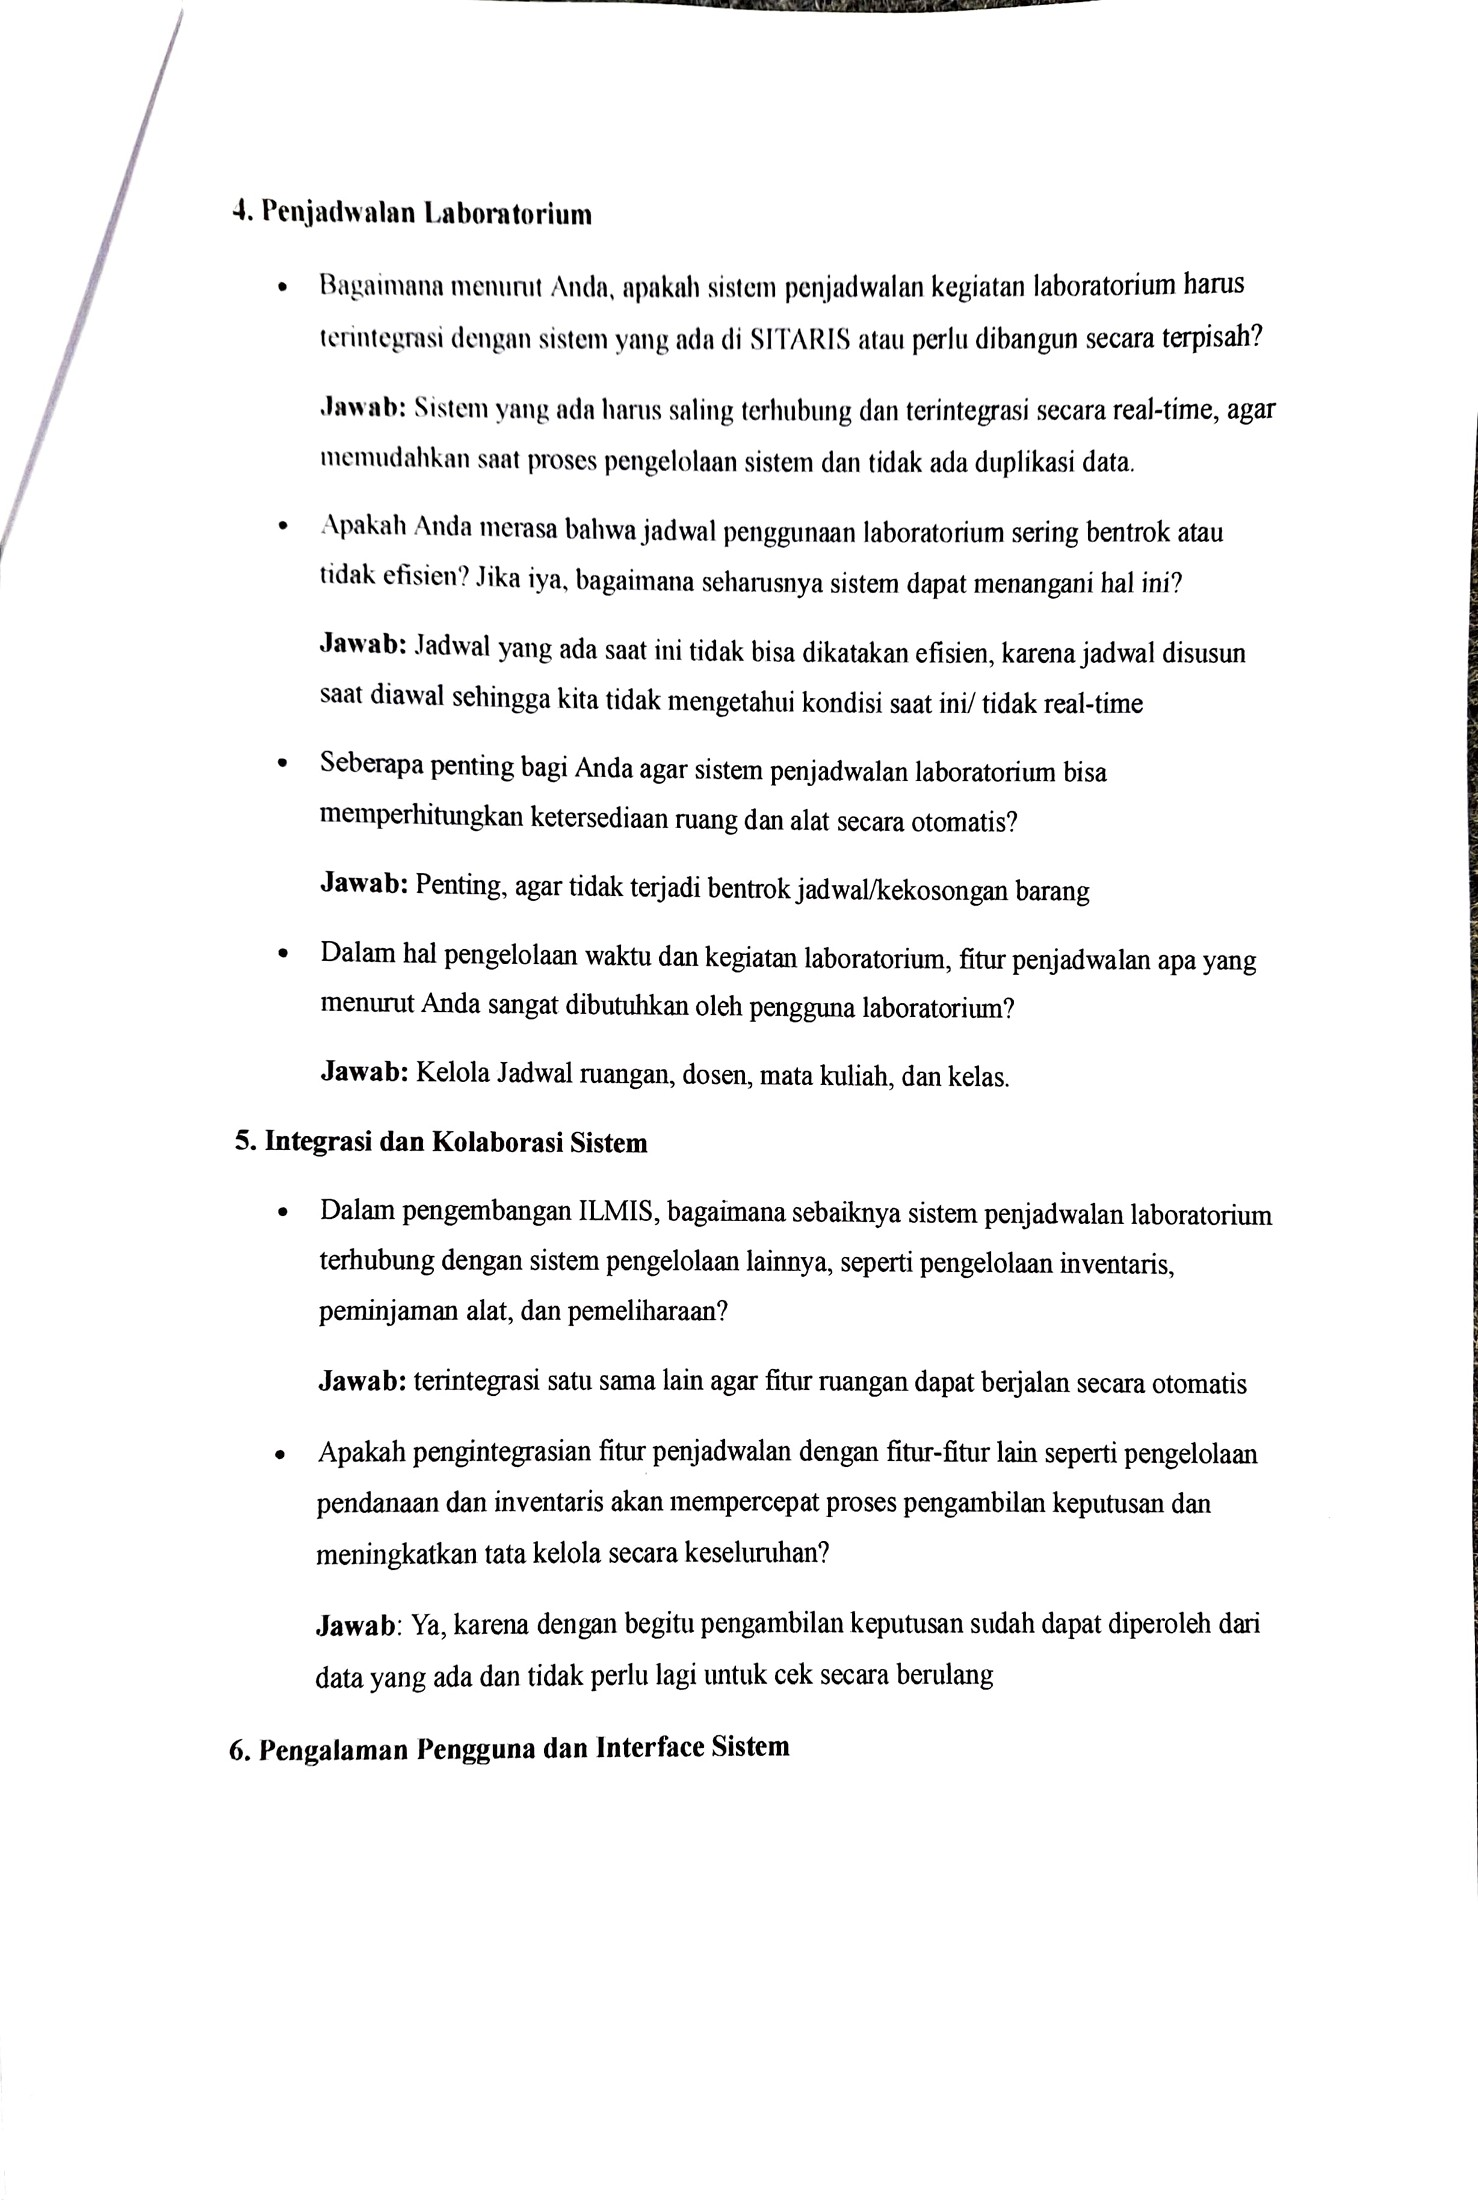
\includegraphics[width=0.82\linewidth]{konten/gambar/wawancara/wawancara_3.jpg}

	\label{fig:hasil-wawancara}
\end{figure}
\begin{figure}[h]
	\centering
	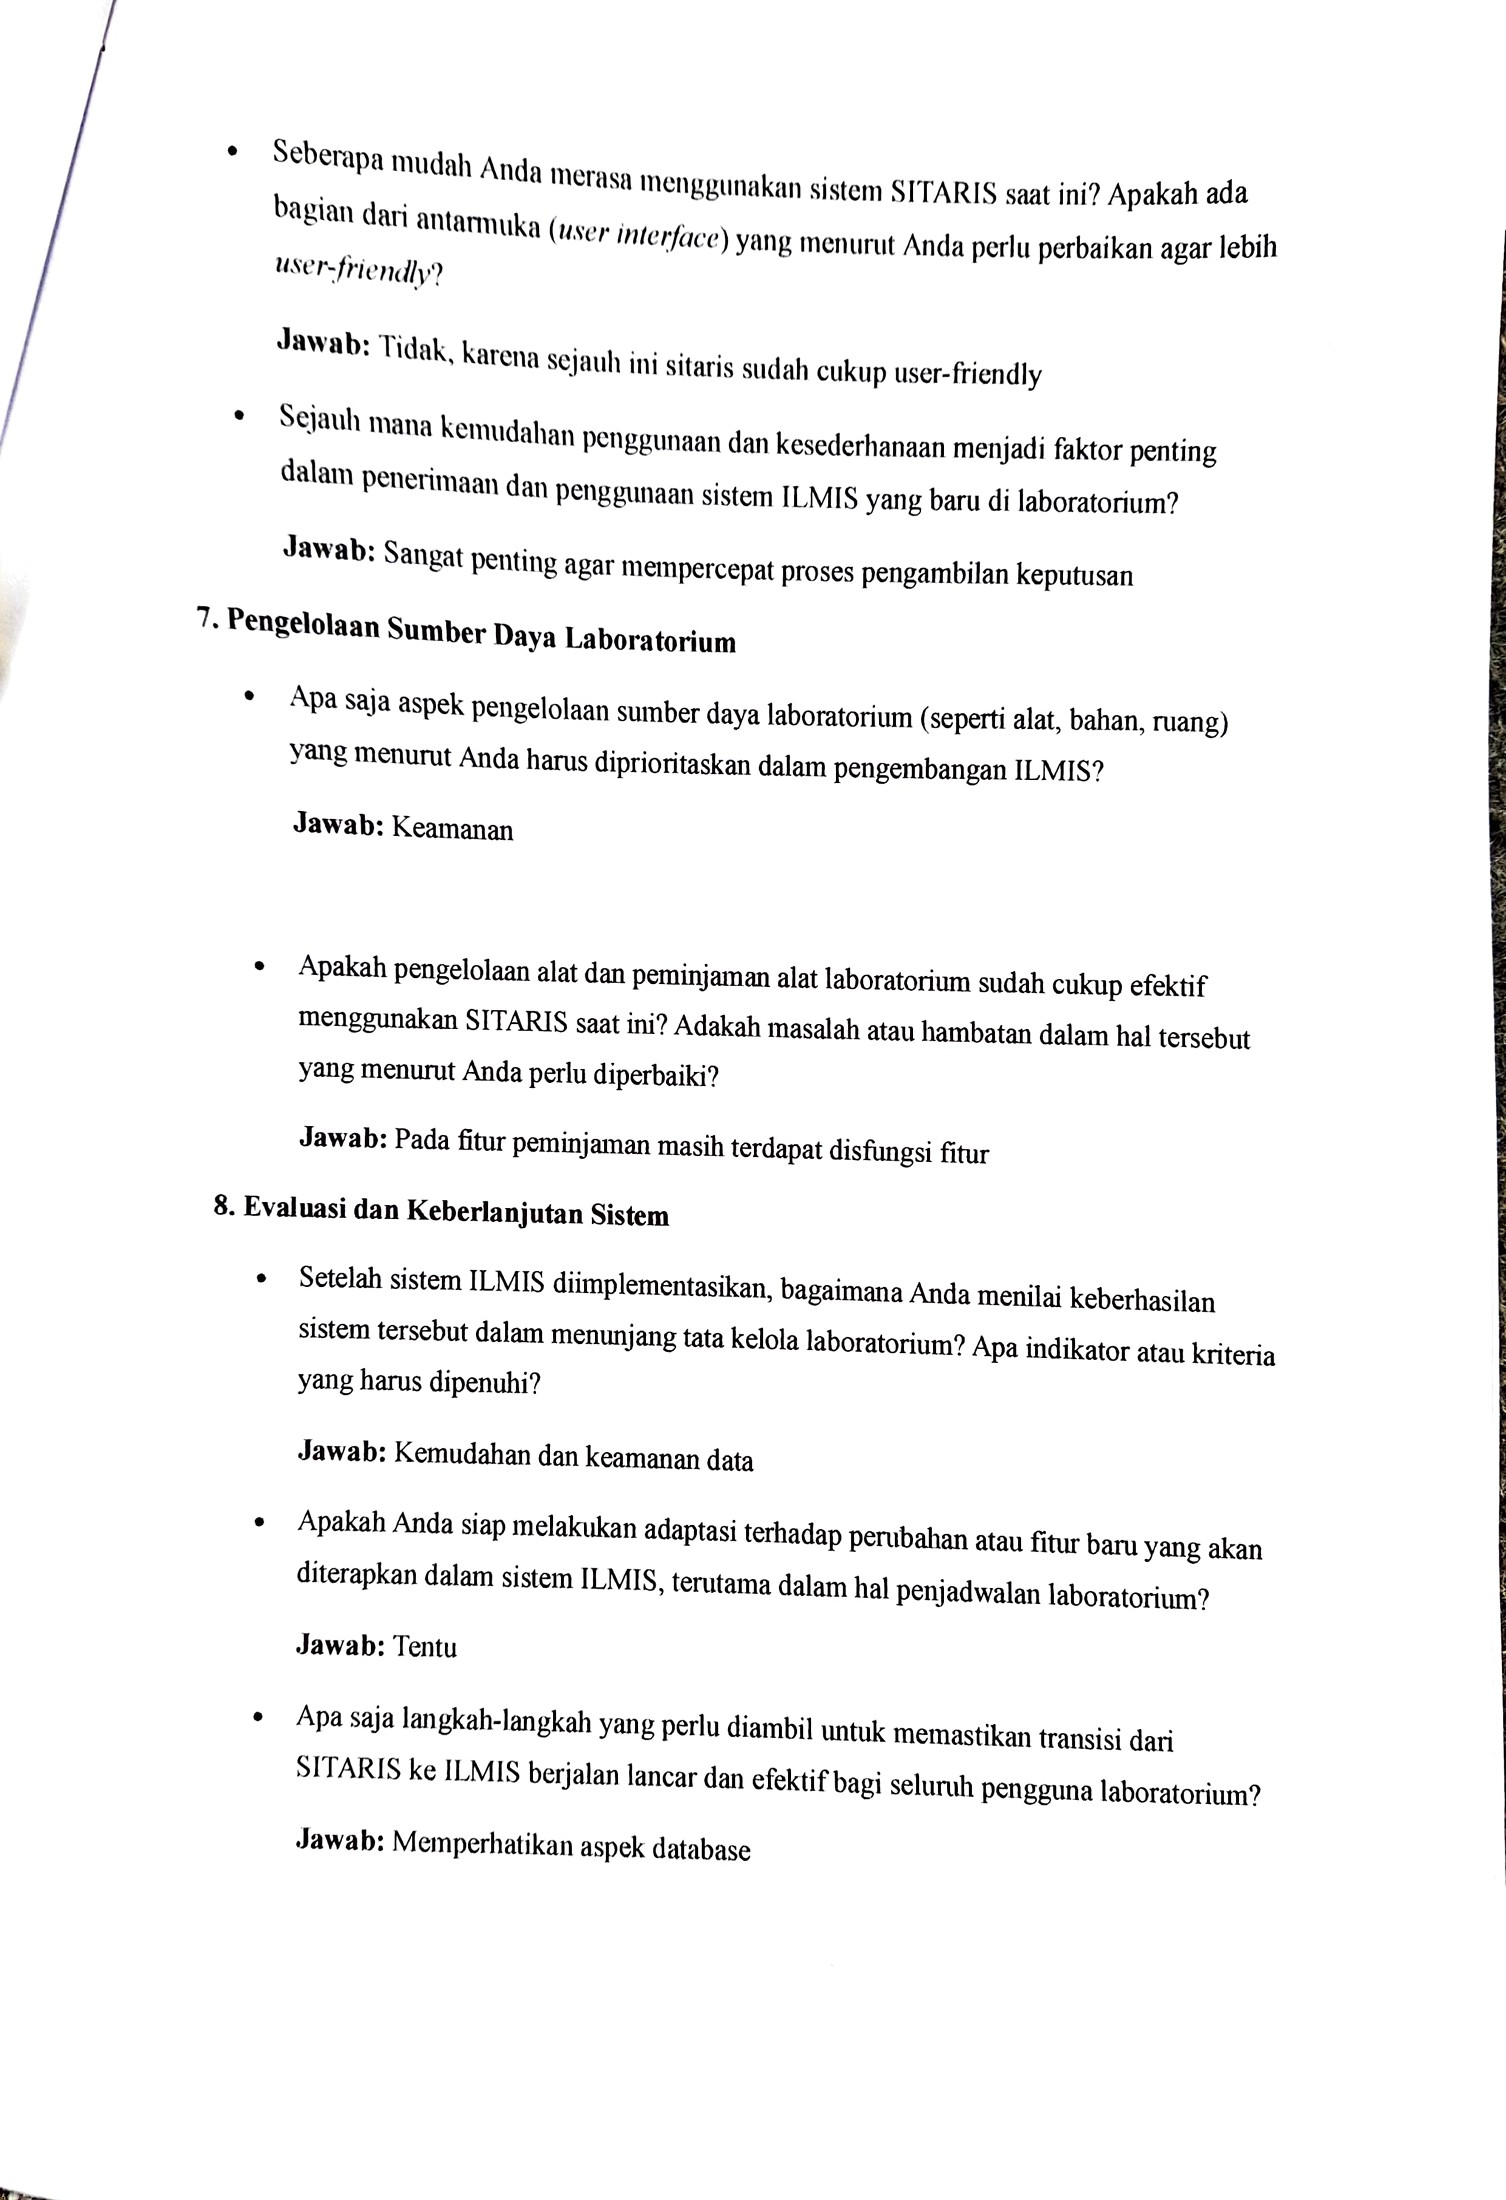
\includegraphics[width=0.82\linewidth]{konten/gambar/wawancara/wawancara_4.jpg}

	\label{fig:hasil-wawancara}
\end{figure}
\begin{figure}[h]
	\centering
	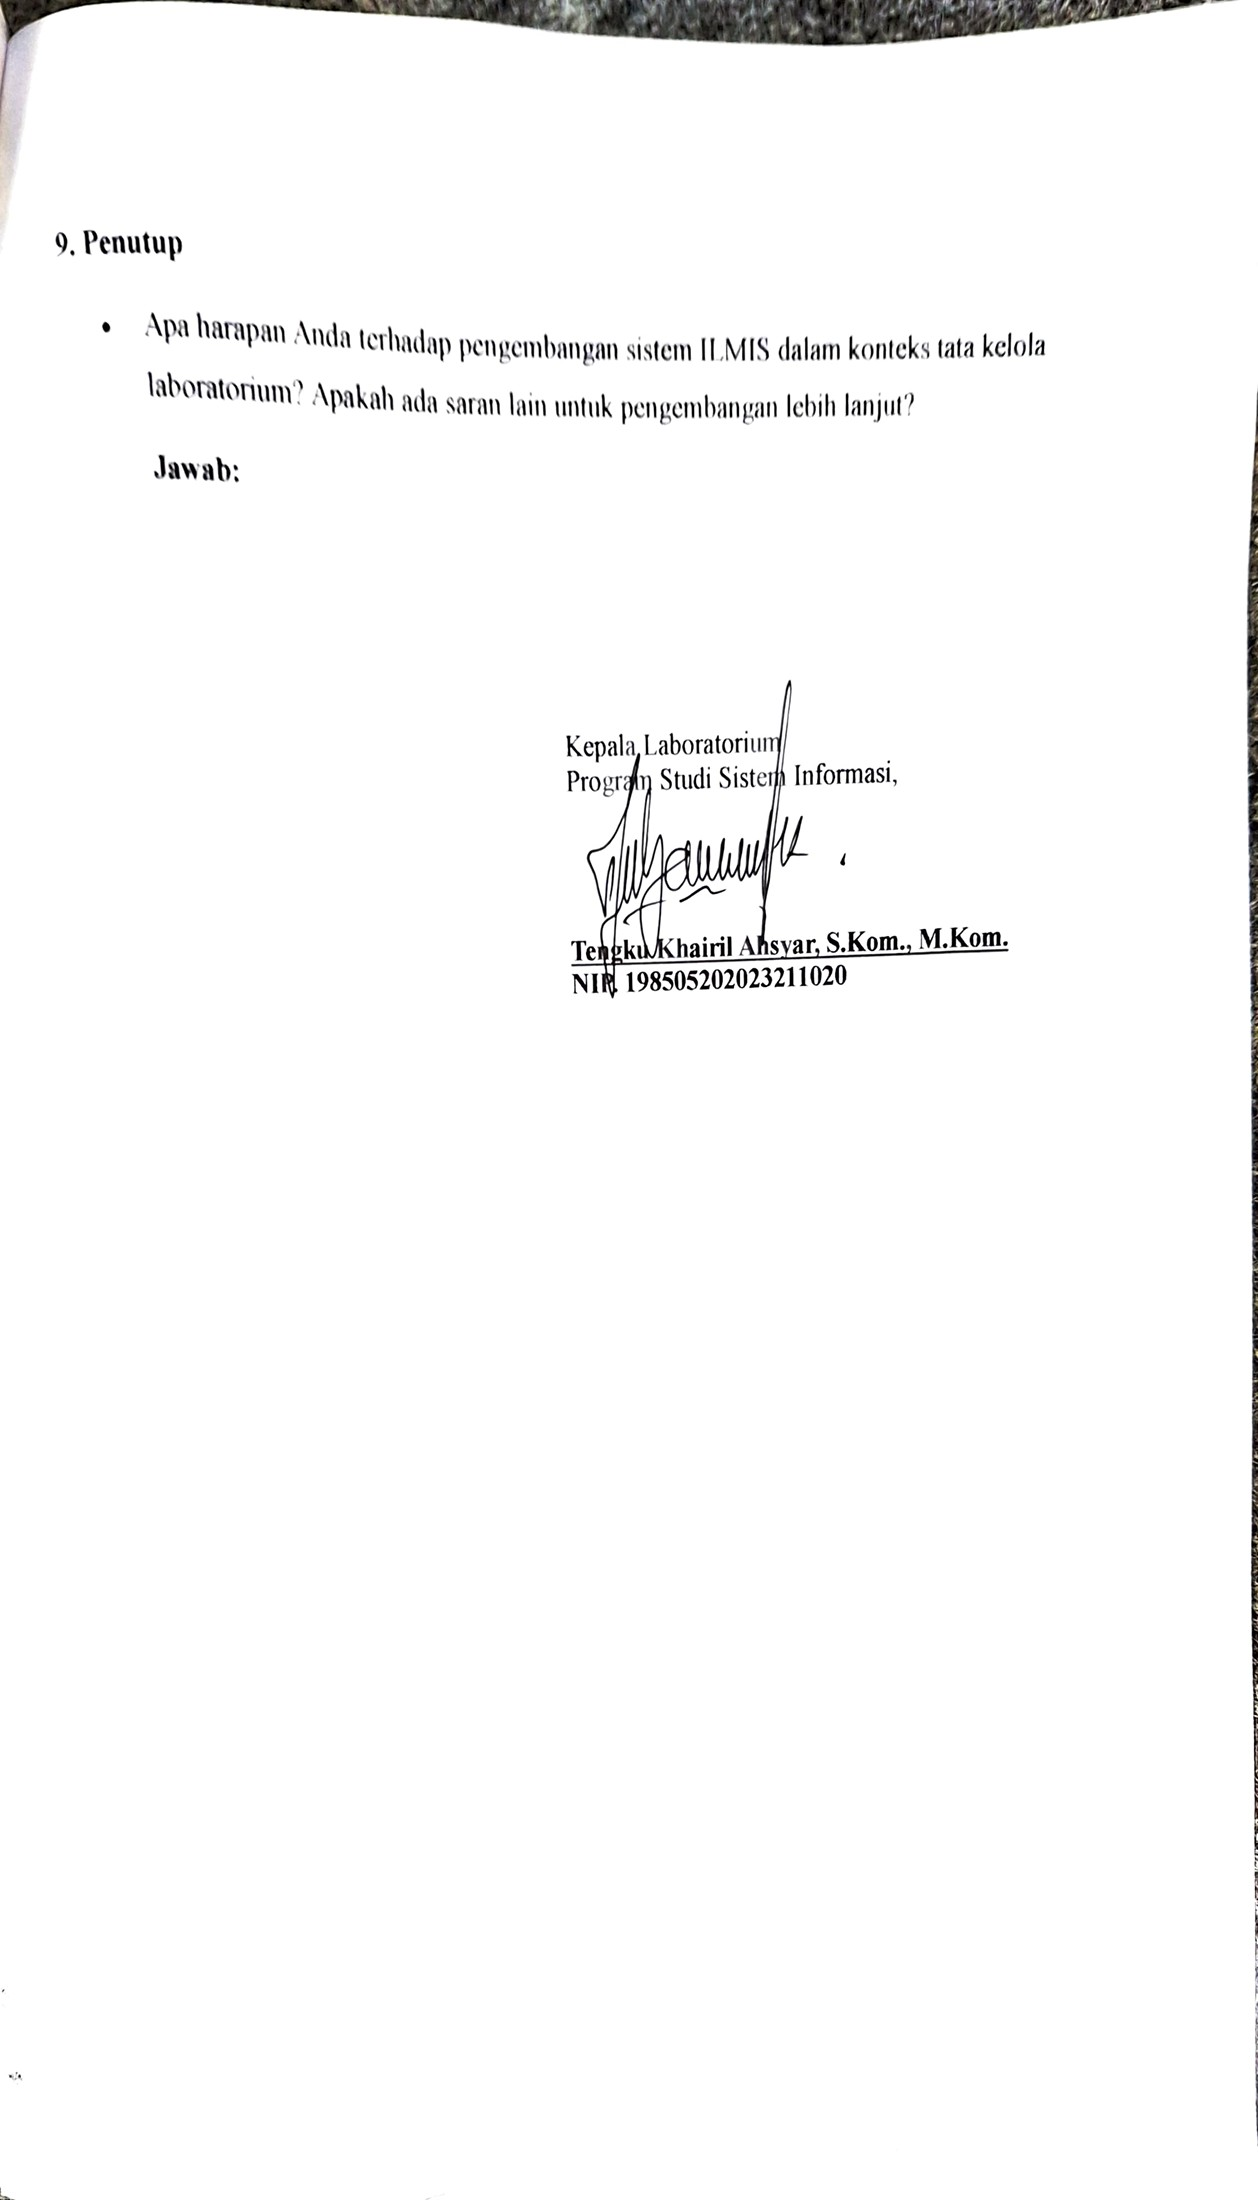
\includegraphics[width=0.82\linewidth]{konten/gambar/wawancara/wawancara_5.jpg}

	\label{fig:hasil-wawancara}
\end{figure}


%-----------------------------------------------------------------------------%
